\section{Univariate Analyse}
Im folgenden Abschnitt wird das vorliegende Datenmaterial des durchschnittlichen Benzinpreises in Deutschland im Rahmen der univariaten Datenanalyse verdichtet, analysiert und ausgewertet.\\

\subsection{Konkretisierung des Merkmals}
\begin{figure}[ht]
  \centering

  \begin{tabular}{| L{0.4\textwidth} | L{0.53\textwidth} |}
    \hline
    \textbf{Merkmal}                  & durchschnittlicher Benzinpreis in Deutschland für 1 Liter Superbenzin                         \\\hline
    \textbf{Merkmalsausprägung} \newline
    (im vorliegenden Datenmaterial)   & Centbeträge im Bereich von 117,1 bis 197,0 Cent je Liter                                      \\\hline
    \textbf{Statistische Masse}                & Stichprobe von 37 Monaten (April, August, Dezember) im Zeitraum von April 2010 bis April 2022 \\\hline
    \textbf{Statistische Einheit}              & ein Monat (April, August oder Dezember)                                                       \\\hline
    \textbf{Merkmalstyp}                       & quasi-stetig                                                                                  \\\hline
    \textbf{Skalenniveau}                      & metrisch verhältnisskaliert                                                                   \\
    \hline
  \end{tabular}
  \caption{Übersicht der Merkmalsbeschreibung}
  \label{tab:tabuebersichtuni}
\end{figure}

Zur Konkretisierung bzw. näheren Erläuterung des Merkmals seien folgende Punkte ergänzt:

\begin{itemize}
  \item Bei dem Merkmal Benzinpreis handelt es sich ausdrücklich nicht um einen konkreten Wert, sondern um den Durchschnittspreis für 1 Liter Superbenzin des betrachteten Monats in Deutschland. Im Folgenden wird aus Gründen der Lesbarkeit auf eine Erwähnung des durchschnittlichen Preises verzichtet und lediglich vom Benzinpreis gesprochen; gemeint ist aber der Durchschnittspreis, sofern nicht anders erwähnt.
  \item Die Stichproben wurden hier jeweils im Abstand von 4 Monaten gewählt; die Werte liegen deshalb für den Monat April, August oder Dezember vor. Eine entsprechende Spezifizierung der statistischen Einheit wurde in der obigen Tabelle vorgenommen.
  \item Die Merkmalsausprägungen können jenseits der Stichprobe selbstverständlich jeden Wert über Null annehmen, wurden aber aufgrund ihrer Vielfältigkeit für die Analyse auf die Spannweite der Stichprobenwerte begrenzt.
\end{itemize}
\pagebreak

\subsection{Verdichtung und Häufigkeitsverteilung}

Bevor die Häufigkeitsverteilung des vorliegenden Datenmaterials untersucht werden kann, wird dieses verdichtet. Da eine Gruppierung der Daten aufgrund zahlreicher, unterschiedlicher Merkmalsausprägungen wenig sinnvoll ist, werden die Daten wie folgt klassiert:

\begin{figure}[ht]
  \centering

\begin{tabular}{l|cccccc}
\textbf{y\textsubscript{j} Bpreis in ct $\cdot$ l\textsuperscript{-1}}        & \textbf{h\textsubscript{j}} & \textbf{f\textsubscript{j}}                  & \textbf{H\textsubscript{j}} & \textbf{F\textsubscript{j}} & \textbf{$\Delta$x\textsubscript{j}} & \textbf{f*\textsubscript{j}} \\ \hline
{[}110;130)            & 6          & 0,1622                      & 6          & 0,1622     & 20               & 0,0081      \\
{[}130;140)            & 8          & 0,2162                      & 14         & 0,3784     & 10               & 0,0216      \\
{[}140;150)            & 10         & 0,2703                      & 24         & 0,6486     & 10               & 0,0270      \\
{[}150;160)            & 9          & 0,2432                      & 33         & 0,8919     & 10               & 0,0243      \\
{[}160;200)            & 4          & 0,1081                      & 37         & 1          & 40               & 0,0027      \\ \hline
$\sum$                      & 37         & 1                           &            &            &                  &
\end{tabular}
\caption{klassierte Datenaufbereitung des durchschnittlichen Benzinpreises}
\label{tab:klassDatenBenz}
\end{figure}


\begin{figure}[H]
  \centering
  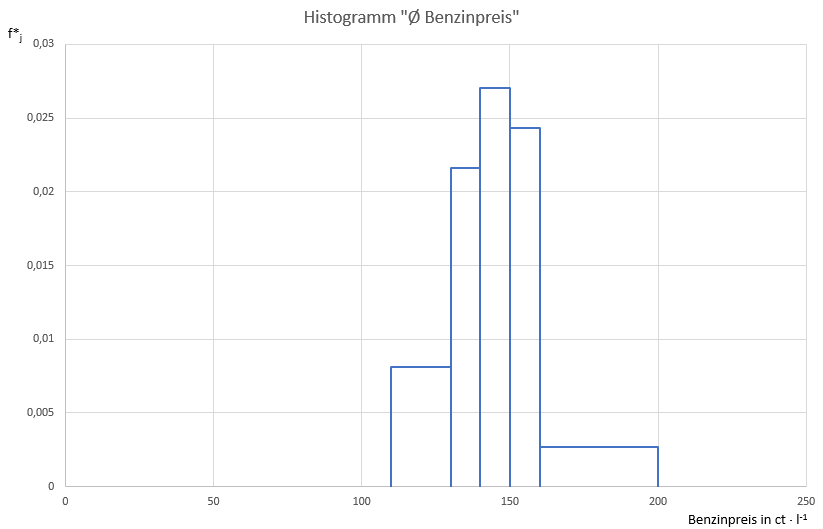
\includegraphics[width = \textwidth]{graphics/histogramm_benz_uni.png}
  \caption{Histogramm "Benzinpreis"}
  \label{fig:histBenzUni}
\end{figure}

\begin{figure}[H]
  \centering
  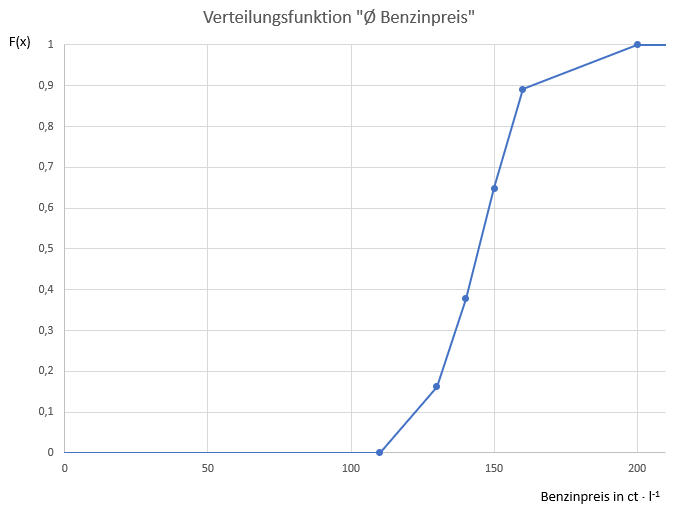
\includegraphics[width = \textwidth]{graphics/verteilungsfunktion.png}
  \caption{Verteilungsfunktion "Benzinpreis"}
  \label{fig:vertBenzUni}
\end{figure}


\subsection{Lageparameter}
Zur Bestimmung des \textbf{Modalwert} werden die Benzinpreis-Daten der Urliste gruppiert und ihre absolute Häufigkeit ermittelt.\\
Dabei lässt sich kein eindeutiger Modalwert bestimmen. Sowohl 141,2 ct $\cdot$ l\textsuperscript{-1} als auch 165,6 ct $\cdot$ l\textsuperscript{-1} treten mit einer absoluten Häufigkeit von 2 auf.\\
Der Modalwert verliert damit an Aussagekraft und wird nicht genauer betrachtet.\\

Um den \textbf{Median} (Zentralwert) zu ermitteln, werden die Benzinpreis-Daten der Urliste der Größe nach sortiert.\\
Da eine Stichprobe im Umfang von 37 Werten vorliegt, ist die Ermittlung ohne viel Aufwand möglich ((37+1)/2 = 19).
Der in der Mitte liegende Wert (x\textsubscript{19}) der Stichprobe ist der Median und beträgt 143,7 ct $\cdot$ l\textsuperscript{-1}.\\

Da das vorliegende Merkmal verhältnisskaliert und damit metrisch ist, kann auch das \textbf{arithmetische Mittel} (1) berechnet werden.\\
Dafür wird die Summe aller erfassten Werte gebildet und durch den Umfang der Stichprobe geteilt:

\begin{equation}
  \bar{x} = \frac{1}{37} \cdot \sum_{i=1}^{37}{x_i} = 144,7 \, \si{\ct\per\liter}
\end{equation}

Dabei ergibt sich ein Mittelwert von 144,7 ct $\cdot$ l\textsuperscript{-1}. Durchschnittlich lag der Benzinpreis im Monat damit bei 144,7 ct $\cdot$ l\textsuperscript{-1}.


\subsection{Streuungsparameter}
In Vorbereitung auf die Analyse der Streuung, werden zunächst das erste und dritte \textbf{Quartil} (2 bis 9) sowie der zwischen ihnen bestehende \textbf{Quartilsabstand} (10) berechnet.

\begin{align}
  (n+1) \cdot p &= (37+1) \cdot 0,25 = 9,5\\
          &g(9,5) = 9; \, nka(9,5) = 0,5
\end{align}

\begin{align}
  x_{0,25} &= (1-0,5) \cdot x_9 + 0,5 \cdot x_{10}\\
        &= 0,5 \cdot 134,5 \, \si{\ct\per\liter} + 0,5 \cdot 135,6 \, \si{\ct\per\liter}\\
        &= 135,050 \, \si{\ct\per\liter}
\end{align}

\begin{align}
  g(28,5) = 28; \, nka(28,5) = 0,5\\
  x_{0,75} &= (1-0,5) \cdot x_{28} + 0,5 \cdot x_{29}\\
        &= 153,200 \, \si{\ct\per\liter}
\end{align}

\begin{align}
 Q = x_{0,75} - x_{0,25} = 153,200 - 135,050 = 18,150 \, \si{\ct\per\liter}
\end{align}


Die mittleren 50\% der untersuchten Monate unterscheiden sich demnach im Benzinpreis um maximal 18,150ct $\cdot$ l\textsuperscript{-1}.\\

Mithilfe des ermittelten Quartilsabstandes kann die vorliegende Datenreihe nun auf \textbf{Ausreißer} untersucht werden. Dafür wird der Quartilsabstand mit dem Faktor 1,5 mutlipliziert und Toleranzgrenzen für die vorliegenden Werte bestimmt:

\begin{align}
 Q \cdot 1,5 = 18,150 \, \si{\ct\per\liter} \cdot 1,5 = 27,225\\
 x_{0,25}: \, 135,050 - 27,225 = 107,825 \, \si{\ct\per\liter}\\
 x_{0,75}: \, 153,200 + 27,255 = 180,425 \, \si{\ct\per\liter}
\end{align}

Werte außerhalb des so definierten Rahmens lassen sich als Ausreißer einordnen; darunter fällt lediglich der Wert 197,0 ct $\cdot$ l\textsuperscript{-1}.\\
Dieser Ausreißer wurde auch in die Berechnung des arithmetischen Mittels einbezogen. Um zu prüfen, ob dieses durch den Ausreißerwert maßgeblich verzerrt wurde, kann das arithmetische Mittel noch einmal nur für die mittleren 50 \% berechnet werden. Dabei ergibt sich ein Wert von \centperliter{144,1}, welcher nur minimal unter dem zuvor berechneten Mittelwert liegt.\\
Der Ausreißer verzerrt damit das arithmetische Mittel leicht nach oben, was bei einer Differenz von 0,6 ct $\cdot$ l\textsuperscript{-1} durchaus vernachlässigbar scheint.\\

Aus den ermittelten Daten kann nun ein Boxplot-Diagramm erstellt werden:

\begin{figure}[H]
  \centering
  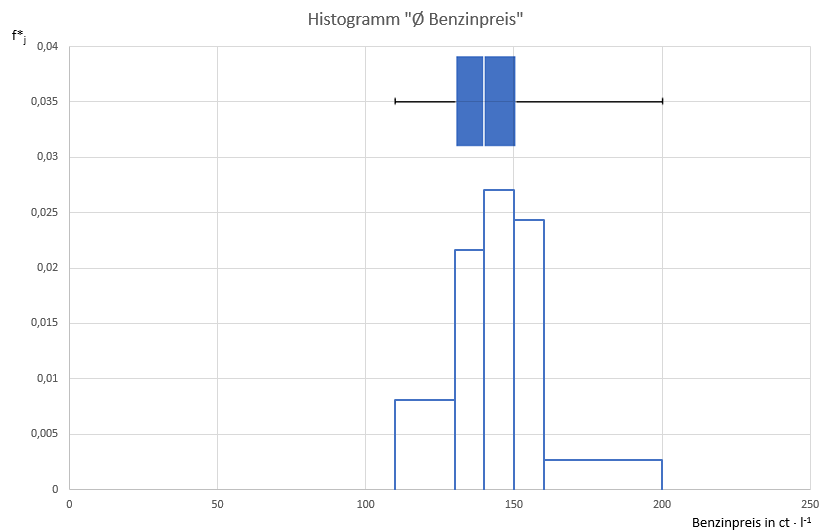
\includegraphics[width = \textwidth]{graphics/histogram_mit_boxplot.png}
  \caption{Histogramm "Benzinpreis" inklusive Boxplot-Diagramm}
  \label{fig:histBoxBenzUni}
\end{figure}

Anhand des Boxplots wird die Verteilung der Werte noch einmal grafisch deutlich. Der Median innerhalb der Box liegt - wenn auch nur minimal - näher am unteren Quartil, die Box ist nicht mittig positioniert, sondern Richtung Minimum verschoben.Die Verteilung ist damit asymmetrisch: \textbf{linkssteil} bzw. rechtsschief.\\
Der Abstand der Merkmalsausprägungen links vom Median ist damit kleiner als der größerer Merkmalsausprägungen rechts vom Median. Zudem fällt das arithmetische Mittel größer als der Zentralwert aus, auch wenn die Differenz nicht sonderlich groß ist (vgl. Median = 143,7 ct $\cdot$ l\textsuperscript{-1}, arithmetisches Mittel = 144,7 ct $\cdot$ l\textsuperscript{-1} und Differenz von 1,0 ct $\cdot$ l\textsuperscript{-1}).\\

Die Verteilung und damit einhergehende Abweichung der Werte lässt sich noch genauer mit der \textbf{Varianz} (14-15) und \textbf{Standardabweichung} (16) untersuchen.\\

\begin{align}
 s_x^2 &= \frac{37}{36} \cdot (\frac{782.266,33}{37}-144,7^2) \, [\si{\ct\per\liter}]^2\\
      &= 222,77697 \, [\si{\ct\per\liter}]^2
\end{align}


Die \textbf{Varianz} $s_x^2$ ist aufgrund ihrer quadratischen Dimension nur schwer mit den bisher ermittelten Werten vergleichbar und lässt keine Interpretation zu. Sie dient lediglich als Zwischenschritt zur Ermittlung der \textbf{Standardabweichung} $s_x$.

\begin{align}
  s_x = \sqrt{222,77697} = 14,926 \, \si{\ct\per\liter}
\end{align}

Die Standardabweichung gewährt nun Einblick in die Streuung der Werte um den Mittelwert. Durchschnittlich weichen die Benzinpreise der betrachteten Monate in der Stichprobe um \centperliter{14,926} vom Mittelwert ab.\\
Das Skalenniveau des Merkmals erlaubt es darüber hinaus, den \textbf{Variationskoeffizienten} (17) zu berechnen und damit die Streuung über die Merkmalsgrenzen hinaus zur allgemeinen Vergleichbarkeit zu quantifizieren:

\begin{align}
  V &= \frac{s_x}{\bar{x}} = \frac{14,926 \, \si{\ct\per\liter}}{144,7 \, \si{\ct\per\liter}} = 0,10318
\end{align}

Prozentual gesehen unterliegen die Benzinpreise damit einer schwachen Streuung von 10,318 \%.

\subsection{Zwischenfazit univariate Datenanalyse}
